\chapter{Manuel de jeu}
\section{Jouer une partie}
Lorsque vous rentrez en jeu, les joueurs et les balles sont placés à leur position initiale. Chaque type de joueur est identifié par une couleur: 
\textbf{bleu} pour les \gls{poursuiveur}s, \textbf{rouge} pour les \gls{batteur}s, \textbf{vert} pour le \gls{gardien} et \textbf{jaune} pour l' 
\gls{attrapeur}. 
Les joueurs aux costumes rayés sont ceux de votre adversaire, les vôtres sont en couleurs pleines.

\subsection{Sélection d'un joueur}
\begin{figure}[h!]
    \centering
    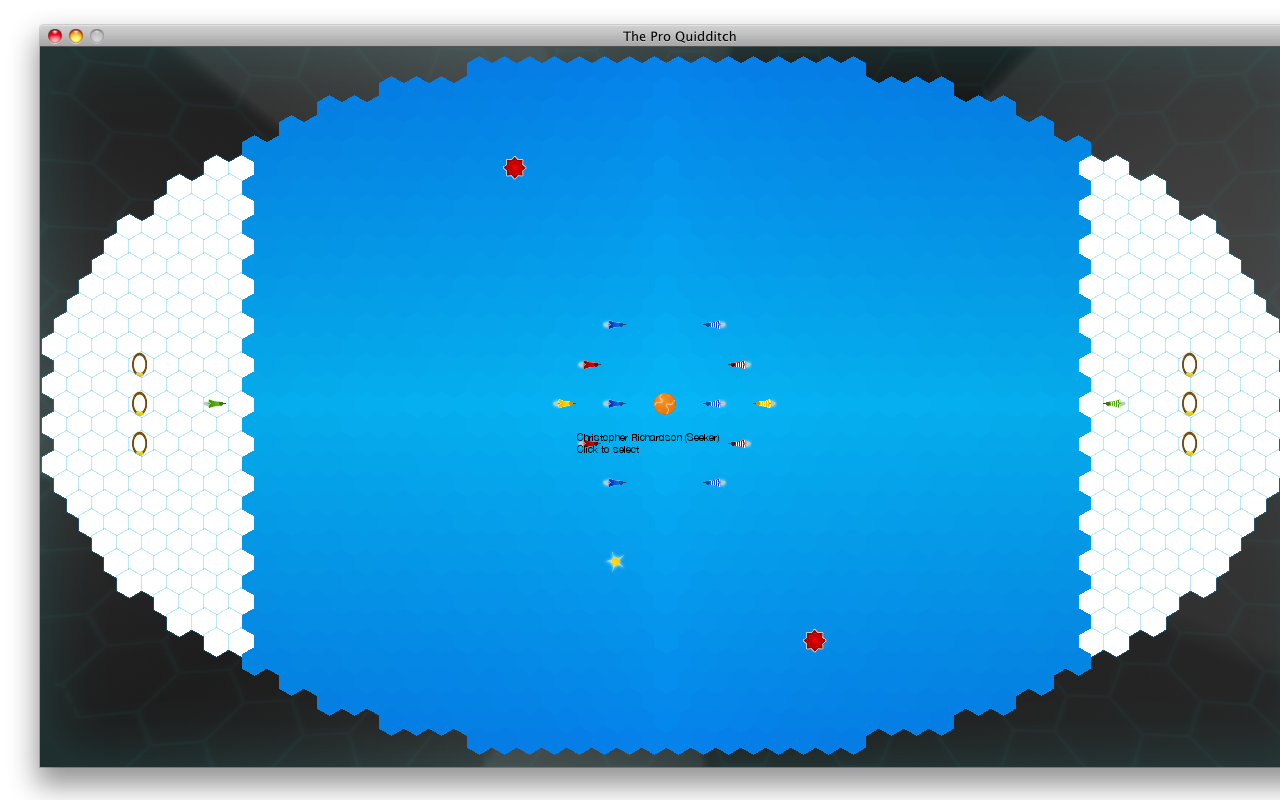
\includegraphics[width=\textwidth]{../screenshots/hover_seeker.png}
    \caption{\label{manual:view_name} Affichage du nom de l'attrapeur lorsque la souris le survole}
\end{figure}

Passez votre souris sur les joueurs pour découvrir leur nom (voir figure \ref{manual:view_name}). Comme l'outil d'aide le suggère, vous pouvez cliquer dessus pour les sélectionner. Une fois votre joueur sélectionné, les cases qu'il peut atteindre sont mises en évidence en jaune. Cliquez sur l'une d'elle: le chemin que parcourera votre joueur est affiché en rouge (voir figure \ref{manual:assign_move}). S'il peut encore continuer, les prochaines cases sont à nouveau mises en évidence en rouge. Pour terminer le mouvement d'un joueur, re-cliquez sur la dernière case atteinte. Le gardien doit toujours rester dans sa zone, et il est interdit de sortir du terrain.

\begin{figure}[h!]
    \centering
    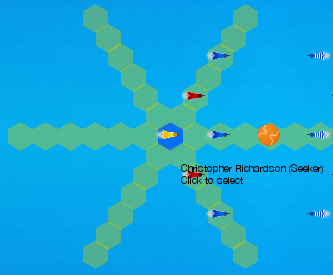
\includegraphics[width=0.45\textwidth]{../screenshots/assign_move.png}
    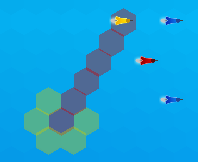
\includegraphics[width=0.45\textwidth]{../screenshots/assign_move2.png}
    \caption{\label{manual:assign_move} Affichage des cases atteignables par un joueur}
\end{figure}

\subsection{Actionner une balle}
Certains joueurs peuvent utiliser des balles. Les poursuiveurs peuvent attraper et lancer le \gls{souaffle}, et les batteurs peuvent taper les 
\gls{cognard}s. Lorsqu'une action de balle a lieu, le déplacement que l'on peut donner à la balle est indiqué en cases bleues.

\subsubsection{Souaffle}
Pour attraper le souaffle, il suffit qu'un poursuiveur ou un gardien passe sur la même case que lui. Quand un joueur est en possession du souaffle, il peut le lancer à toute case de son déplacement, en cliquant-droit sur la dernière position atteinte (indiquée en rouge). Les cases sur lesquelles il peut lancer la balle sont alors indiquées en bleu.

\begin{figure}[h!]
    \centering
    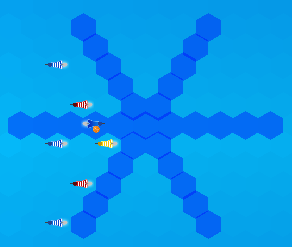
\includegraphics[width=0.5\textwidth]{../screenshots/throw_quaffle.png}
    \caption{\label{manual:throw_quaffle} Lancement du souaffle}
\end{figure}


\subsubsection{Cognards}
Pour lancer un cognard avec un batteur, il suffit de déplacer ce dernier sur la case de la balle. En cliquant sur la case de la balle, les marqueur bleus apparaîtront, vous permettant de battre la balle.

\begin{figure}[h!]
    \centering
    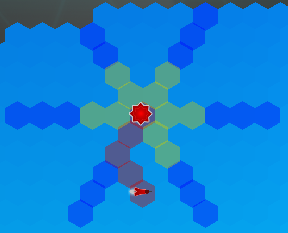
\includegraphics[width=0.5\textwidth]{../screenshots/throw_bludger.png}
    \caption{\label{manual:throw_bludger} Taper sur un cognard}
\end{figure}
